\documentclass[tikz,border=3.14mm]{standalone}
\usepackage{amsmath}
\usetikzlibrary{matrix,decorations.pathreplacing}
\usepackage{graphicx}

\begin{document}
	
	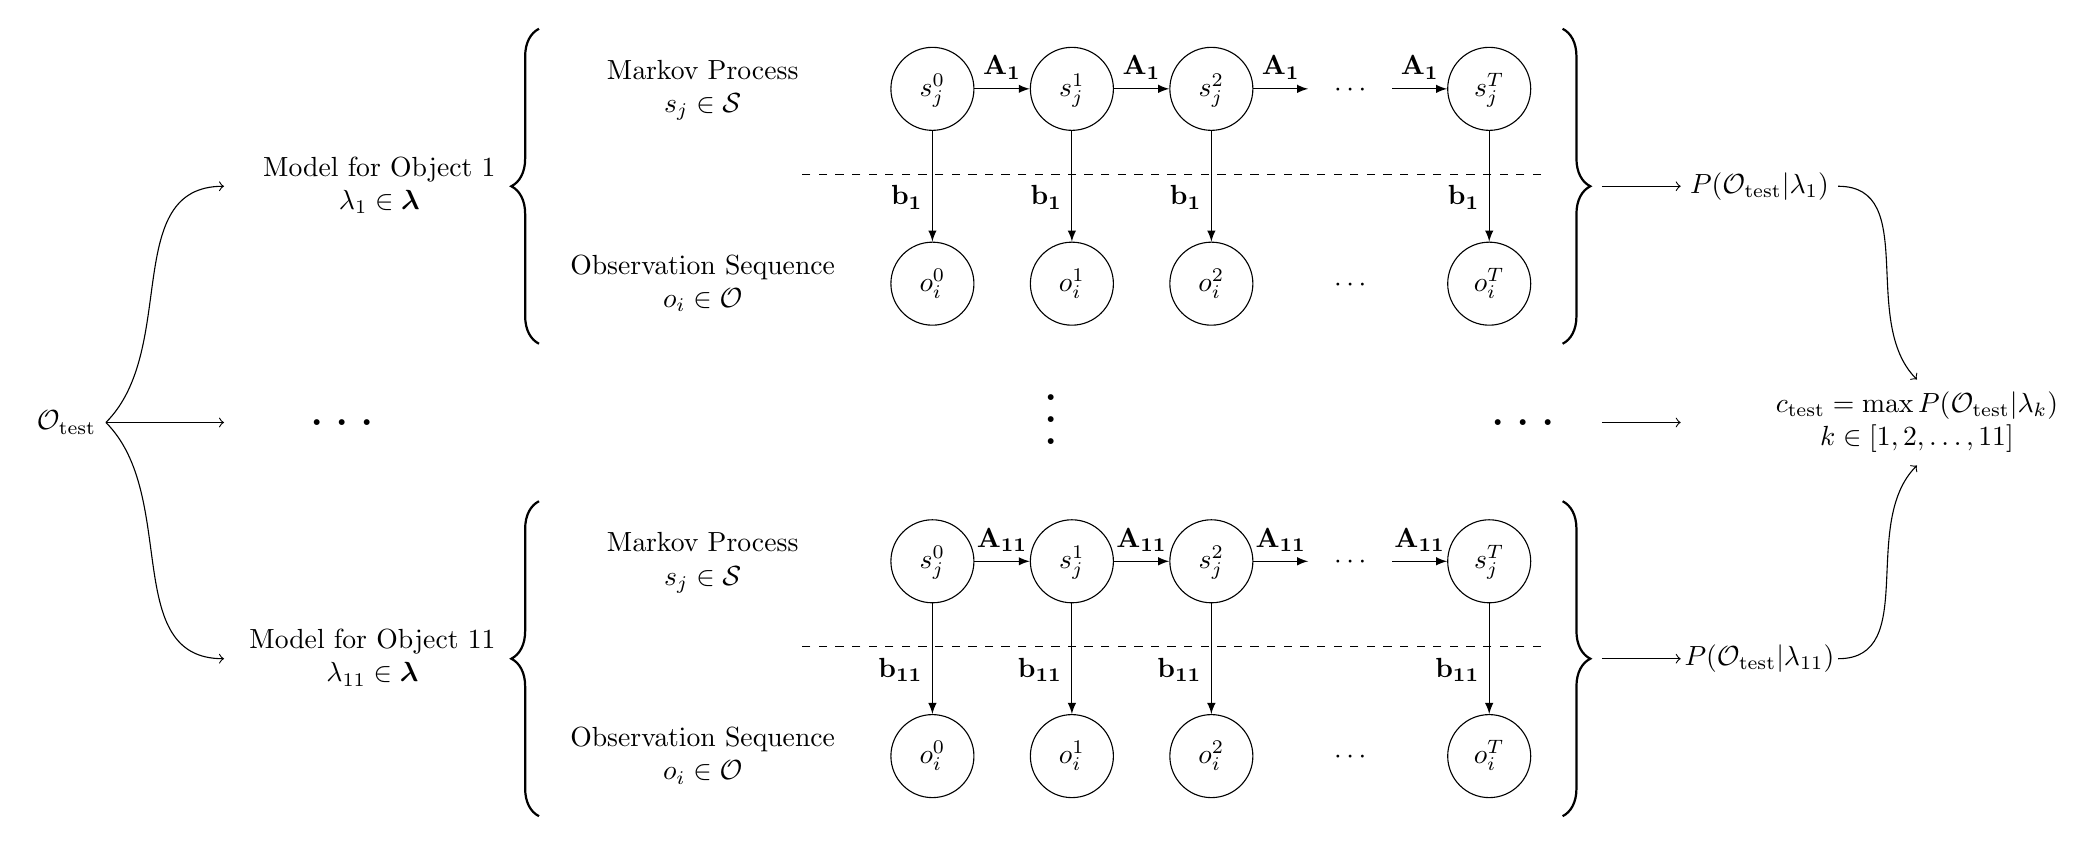
\begin{tikzpicture}
		\matrix (m1) at (0,0) [matrix of math nodes,column sep=2em,row sep=4em,
		cells={nodes={circle,draw,minimum width=3em,inner sep=0pt,
				text height=1.5ex,text depth=0.25ex}},
		column 1/.style={nodes={rectangle,draw=none}},
		column 5/.style={nodes={rectangle,draw=none}},
		nodes in empty cells] (m) {
			\text{$\begin{matrix}\text{Markov Process}\\\text{$s_j \in \mathcal{S}$}\end{matrix}$} & s_j^{0} & s_j^{1} & s_j^{2} & \cdots & s_j^{T}\\
			\text{$\begin{matrix}\text{Observation Sequence}\\\text{$o_i \in \mathcal{O}$}\end{matrix}$} & o_i^0 & o_i^1 & o_i^2 & \cdots & o_i^{T}\\
		};
		\foreach \X in {2,3,4,5} {
			\draw [-latex] (m-1-\X) -- (m-1-\the\numexpr\X+1) node [midway,above] {$\mathbf{A_1}$};
			\ifnum\X=5
			\draw [-latex] (m-1-6) -- (m-2-6) node [pos=0.6,left] {$\mathbf{b_1}$};
			\else
			\draw [-latex] (m-1-\X) -- (m-2-\X) node [pos=0.6,left] {$\mathbf{b_1}$};
			\fi
		}
		\draw [dashed] ([yshift=1ex]m.east) -- ([yshift=1ex]m.east-|m-1-1.east);
		
		% Add big square brackets
		\draw [thick, decorate, decoration={brace,amplitude=10pt, mirror}] (-6.5,2) -- (-6.5,-2) node[midway,left=12pt] {$\begin{matrix}\text{Model for Object 1}\\\text{$\lambda_1 \in \boldsymbol{\lambda}$}\end{matrix}$};
		\draw [thick, decorate, decoration={brace,amplitude=10pt}] (6.5, 2) -- (6.5, -2);
		
		\node at (0,-2.75) {\scalebox{2}{$\vdots$}};
		
		\matrix (m1) at (0,-6) [matrix of math nodes,column sep=2em,row sep=4em,
		cells={nodes={circle,draw,minimum width=3em,inner sep=0pt,
				text height=1.5ex,text depth=0.25ex}},
		column 1/.style={nodes={rectangle,draw=none}},
		column 5/.style={nodes={rectangle,draw=none}},
		nodes in empty cells] (m) {
			\text{$\begin{matrix}\text{Markov Process}\\\text{$s_j \in \mathcal{S}$}\end{matrix}$} & s_j^{0} & s_j^{1} & s_j^{2} & \cdots & s_j^{T}\\
			\text{$\begin{matrix}\text{Observation Sequence}\\\text{$o_i \in \mathcal{O}$}\end{matrix}$} & o_i^0 & o_i^1 & o_i^2 & \cdots & o_i^{T}\\
		};
		\foreach \X in {2,3,4,5} {
			\draw [-latex] (m-1-\X) -- (m-1-\the\numexpr\X+1) node [midway,above] {$\mathbf{A_{11}}$};
			\ifnum\X=5
			\draw [-latex] (m-1-6) -- (m-2-6) node [pos=0.6,left] {$\mathbf{b_{11}}$};
			\else
			\draw [-latex] (m-1-\X) -- (m-2-\X) node [pos=0.6,left] {$\mathbf{b_{11}}$};
			\fi
		}
		\draw [dashed] ([yshift=1ex]m.east) -- ([yshift=1ex]m.east-|m-1-1.east);
		
		% Add big square brackets
		\draw [thick, decorate, decoration={brace,amplitude=10pt, mirror}] (-6.5,-4) -- (-6.5,-8) node[midway,left=12pt] {$\begin{matrix}\text{Model for Object 11}\\\text{$\lambda_{11} \in \boldsymbol{\lambda}$}\end{matrix}$};
		\draw [thick, decorate, decoration={brace,amplitude=10pt}] (6.5,-4) -- (6.5,-8);
		
		% Add arrows pointing to models
		\draw[->] (-12,-3) to [out=45, in=180] (-10.5,0);
		\draw[->] (-12,-3) to [out=-45, in=-180] (-10.5,-6);
		\draw[->] (-12,-3) -- (-10.5,-3);
		\node (dots) at (-9,-3) {\scalebox{2}{$\hdots$}};
		\node (input) at (-12.5,-3) {$\mathcal{O}_{\text{test}}$};
		
		\draw[->] (7,0) -- (8,0);
		\draw[->] (7,-6) -- (8,-6);
		\node (input) at (9,0) {$P(\mathcal{O}_{\text{test}}|\lambda_{1})$};
		\node (input) at (9,-6) {$P(\mathcal{O}_{\text{test}}|\lambda_{11})$};
		
		\node (output) at (11,-3) {$\begin{matrix}c_{\text{test}}=\max P(\mathcal{O}_{\text{test}}|\lambda_{k})\\k \in [1,2,\dots,11]\end{matrix}$};
		
		\draw[->] (10,0) to [out=0, in=135] (output.north);
		\draw[->] (10,-6) to [out=0, in=-135] (output.south);
		
		\draw[->] (7,-3) -- (8,-3);
		\node (dots) at (6,-3) {\scalebox{2}{$\hdots$}};
		
	\end{tikzpicture}
	
\end{document}
